\documentclass[12pt]{article}

% --- Packages ---
\usepackage[utf8]{inputenc}
\usepackage[T1]{fontenc}
\usepackage[french]{babel}
\usepackage{amsmath, amssymb}
\usepackage{geometry}
\usepackage{tikz}
\usepackage[most]{tcolorbox}
\usepackage{lmodern}
\usepackage{tkz-tab}
\usepackage{enumitem}
\usepackage{multicol}
\usepackage{pgfplots}
\pgfplotsset{compat=1.18}
\usepackage{mdframed}
\usepackage{bm}
\usepackage{xcolor}
\usepackage{sectsty}
\usepackage[utf8]{inputenc}
\usepackage[T1]{fontenc}
\usepackage[dvipsnames]{xcolor}
\usepackage{tkz-tab}
\usepackage{multido}

% --- Page ---
\geometry{margin=2cm}

% Footer
\usepackage{fancyhdr}
\pagestyle{fancy}
\cfoot{\thepage}
\rfoot{\textit{G.M.}}
\renewcommand{\headrulewidth}{0pt}
\renewcommand{\footrulewidth}{0pt}

\usetikzlibrary{shapes.misc}

\tikzset{cross/.style={cross out, draw=black, minimum size=2*(#1-\pgflinewidth), inner sep=0pt, outer sep=0pt},
%default radius will be 1pt.
cross/.default={4pt}}

% Pour les titres
\usepackage{sectsty}
\setlength{\parindent}{0pt}
\sectionfont{\color{red}\Large\bfseries}

\begin{document}

% ============================
%   Dérivation
% ============================

\begin{center}
    {\LARGE \textbf{Dérivation}}\\[4mm]
    {\large 1ère STMG}
\end{center}

\hrule
\vspace{0.4cm}

% ============================
%   PARTIE 1 : Nombre dérivé
% ============================

\section*{\textcolor{red}{Partie 1 : Nombre dérivé}}

\subsection*{\textcolor{red}{\hspace{1cm}1) Rappel : coefficient directeur d'une droite}}

\vspace{5pt}

\underline{Rappel :}
\vspace{10pt}
\\Soit une droite passant par les points $A(x_A, y_A)$ et $B(x_B, y_B)$.
\\Le coefficient directeur de cette droite est donné par :
\[
a = \dfrac{\Delta y}{\Delta x} = \dfrac{f(b) - f(a)}{b - a} = \frac{y_B - y_A}{x_B - x_A}
\]

{\color{red}Ce coefficient directeur est également appelé \textbf{taux 
de variation} de $f$.

\vspace{5pt}
Il représente \textbf{la pente} de la droite $(AB)$.}

\vspace{10pt}

\underline{Exemple :}

\vspace{-10pt}

\begin{minipage}[t]{.35\textwidth}%
    \vspace{20pt}

    Le coefficient directeur de la droite $(AB)$ est égal à :

    \vspace{20pt}
    \hspace{10pt}$a_{AB} = $

    \vspace{30pt}

    Le coefficient directeur de la droite $(CD)$ est égal à :

    \vspace{20pt}
    \hspace{10pt}$a_{CD} = $
\end{minipage}%
\hfill
\begin{minipage}[t]{.55\textwidth}%
    \vspace{0pt}
    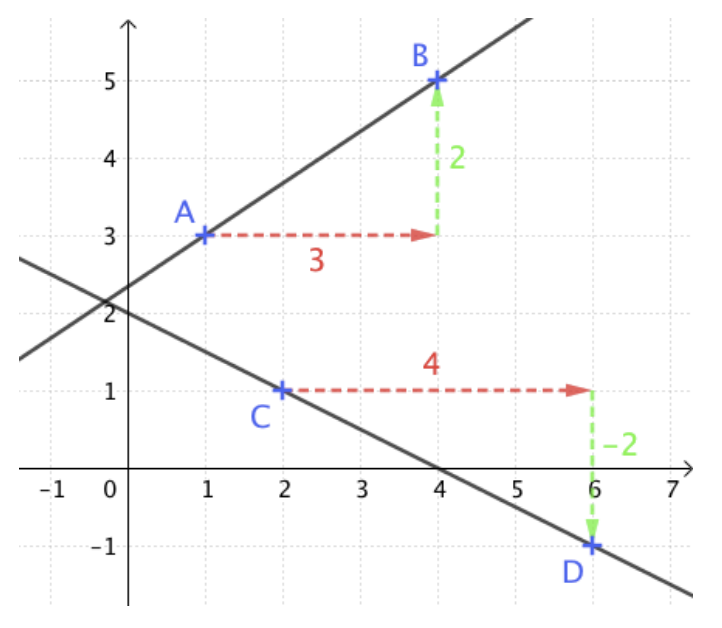
\includegraphics[width=0.8\textwidth]{coefdir.png}
\end{minipage}%


\begin{mdframed}[
    linewidth=1pt,
    roundcorner=5pt,
    linecolor=RoyalBlue,
    innertopmargin=10pt,
    innerbottommargin=10pt
]
{\color{RoyalBlue}\textbf{\underline{Exercice d'application n°1 :} Calculer un coefficient directeur.}}
\vspace{5pt}
\\
\begin{minipage}[t]{.45\textwidth}%
    \vspace{10pt}
    Pour chacune des droites représentées, donner le vecteur directeur.
\end{minipage}%
\hfill
\begin{minipage}[t]{.45\textwidth}%
    \vspace{0pt}
    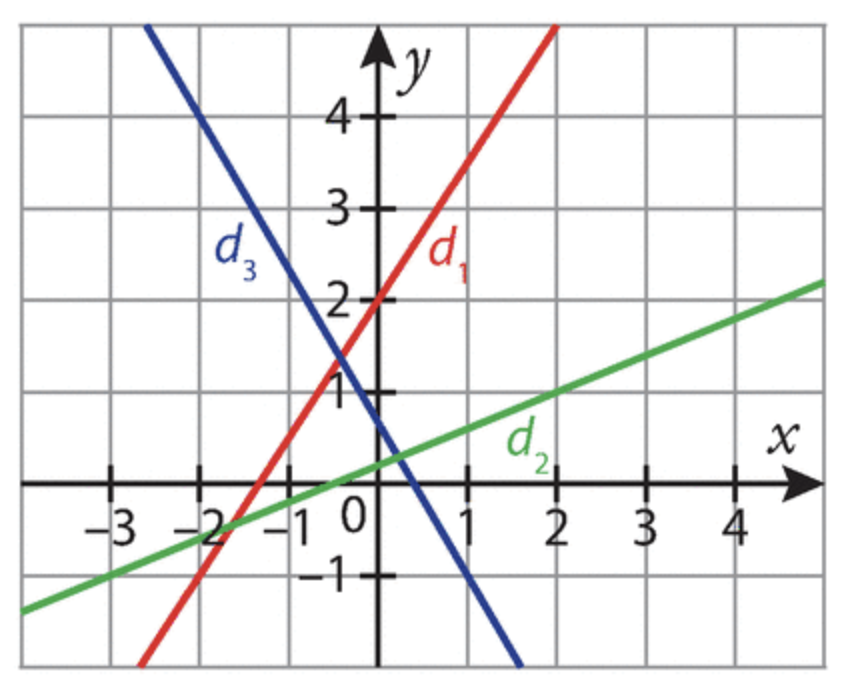
\includegraphics[width=0.7\textwidth]{coefdirexo.png}
\end{minipage}%
\end{mdframed}

\vspace{20pt}

\subsection*{\textcolor{red}{\hspace{1cm}2) Taux de variation}}

\vspace{10pt}

\begin{mdframed}[
    linewidth=1pt,
    roundcorner=5pt,
    linecolor=ForestGreen
]
{\color{ForestGreen}\textbf{Définition :}}
Soit $f$ une fonction. Soient $a$ et $b$ deux nombres réels distincts.

\vspace{5pt}
On appelle \textbf{taux de variation de $\bm{f}$ entre $\bm{a}$ et $\bm{b}$} le nombre : 
\[
\tau = \dfrac{f(b)-f(a)}{b-a}
\]
\end{mdframed}

\vspace{5pt}

\underline{Exemple :}
\\
Soit $f$ la fonction qui, à tout $x$, associe le nombre $f(x) = x^2$.

Le taux de variation de $f$ entre les valeurs 2 et 3 est :

\vspace{30pt}
\hspace{2cm}$\tau = $

\vspace{30pt}

\begin{mdframed}[
    linewidth=1pt,
    roundcorner=5pt,
    linecolor=RoyalBlue,
    innertopmargin=10pt,
    innerbottommargin=10pt
]
{\color{RoyalBlue}\textbf{\underline{Exercice d'application n°2 :} Calculer le taux de 
variation d'une fonction.}}

\vspace{10pt}
Soit $f$ la fonction qui, à tout $x$, associe le nombre $f(x) = x^3$.

\vspace{5pt}
Calculer le taux de variation de la fonction entre 1 et 3.
\end{mdframed}

\vspace{10pt}

\subsection*{\textcolor{red}{\hspace{1cm}3) Fonction dérivable}}

\vspace{5pt}

\underline{Exemple :}

\vspace{-30pt}

\begin{minipage}[t]{.45\textwidth}%
    \vspace{30pt}
    Sur le graphique ci-contre, la pente (coefficient directeur) de la droite $(AM)$ 
    \textbf{sécante à la courbe} est égale à :
    \[
    \dfrac{f(a+h)-f(a)}{(a+h)-a} = \dfrac{f(a+h)-f(a)}{h} , \quad \text{avec } h \neq 0
    \]

    {\color{red}Lorsque $M$ se rapproche de $A$, $h$ se rapproche de $0$ (on note $h 
    \rightarrow 0$)
    
    \vspace{5pt}
    Lorsque h est très proche de 0, la droite (AM) 
    se rapproche d'une position dont la pente est égale à la dérivée de $f$ en $a$.
    }
\end{minipage}%
\hfill
\begin{minipage}[t]{.48\textwidth}%
    \vspace{0pt}
    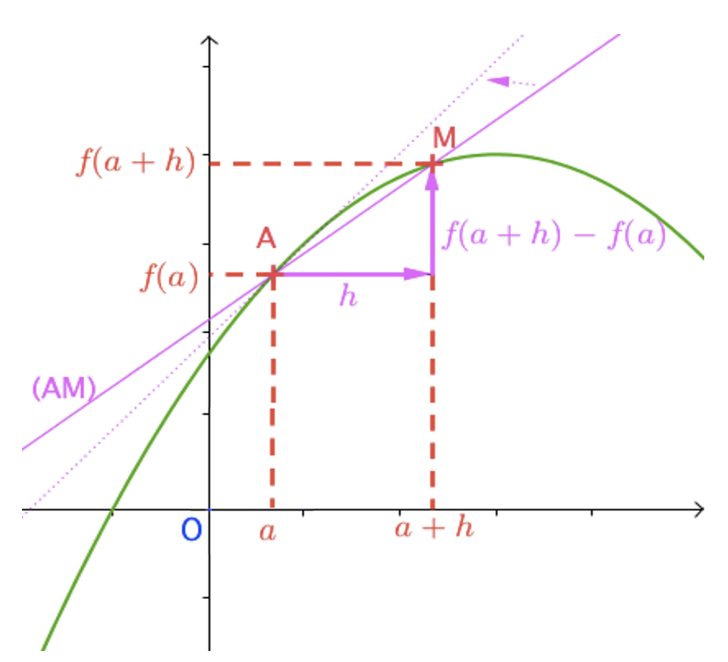
\includegraphics[width=1\textwidth]{taux_acc.png}
\end{minipage}%

\begin{center}
    {\color{red}\fbox{
        \parbox{0.6\textwidth}{
        On note \underline{la pente de cette droite} au point 
        d'abscisse $a$ :
        \[\bm{f'(a)}\]
        
        C'est le nombre dérivé de $f$ en $a$.}}}
\end{center}

On a alors : $f'(a) = \lim\limits_{h \to 0}\dfrac{f(a+h)-f(a)}{h}$, on parle ici de limite 
quand \textbf{$\bm{h}$ tend vers 0}.

\vspace{20pt}

% ============================
%   PARTIE 2 : Tangente à une courbe
% ============================

\section*{\textcolor{red}{Partie 2 : Tangente à une courbe}}

\subsection*{\textcolor{red}{\hspace{1cm}1) Définition}}

\vspace{-30pt}

\begin{minipage}[t]{.45\textwidth}%
    \vspace{60pt}
    \begin{mdframed}[
        linewidth=1pt,
        roundcorner=5pt,
        linecolor=ForestGreen
    ]
    {\color{ForestGreen}\textbf{Définition :}}
    Une \textbf{tangente} à une courbe est une droite qui « touche » la 
    \vspace{5pt}\\
    courbe en 
    \_\_\_\_\_\_\_\_\_\_\_\_\_\_\_\_.
    \end{mdframed}
\end{minipage}%
\hfill
\begin{minipage}[t]{.45\textwidth}%
    \vspace{0pt}
    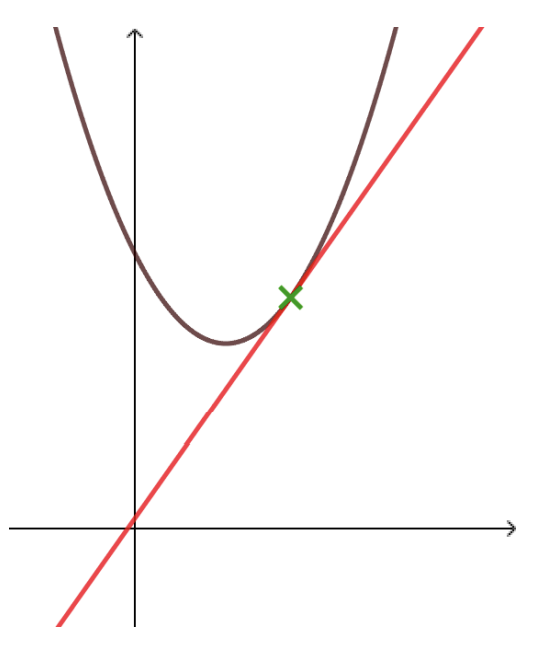
\includegraphics[width=0.7\textwidth]{tangente.png}
\end{minipage}%


\vspace{10pt}

\subsection*{\textcolor{red}{\hspace{1cm}2) Coefficient directeur de la tangente}}

\vspace{-10pt}

\begin{minipage}[t]{.45\textwidth}%
    \vspace{60pt}
    $A$ est un point d'abscisse $a$ appartenant à la courbe représentative de la fonction $f$.
\end{minipage}%
\hfill
\begin{minipage}[t]{.45\textwidth}%
    \vspace{0pt}
    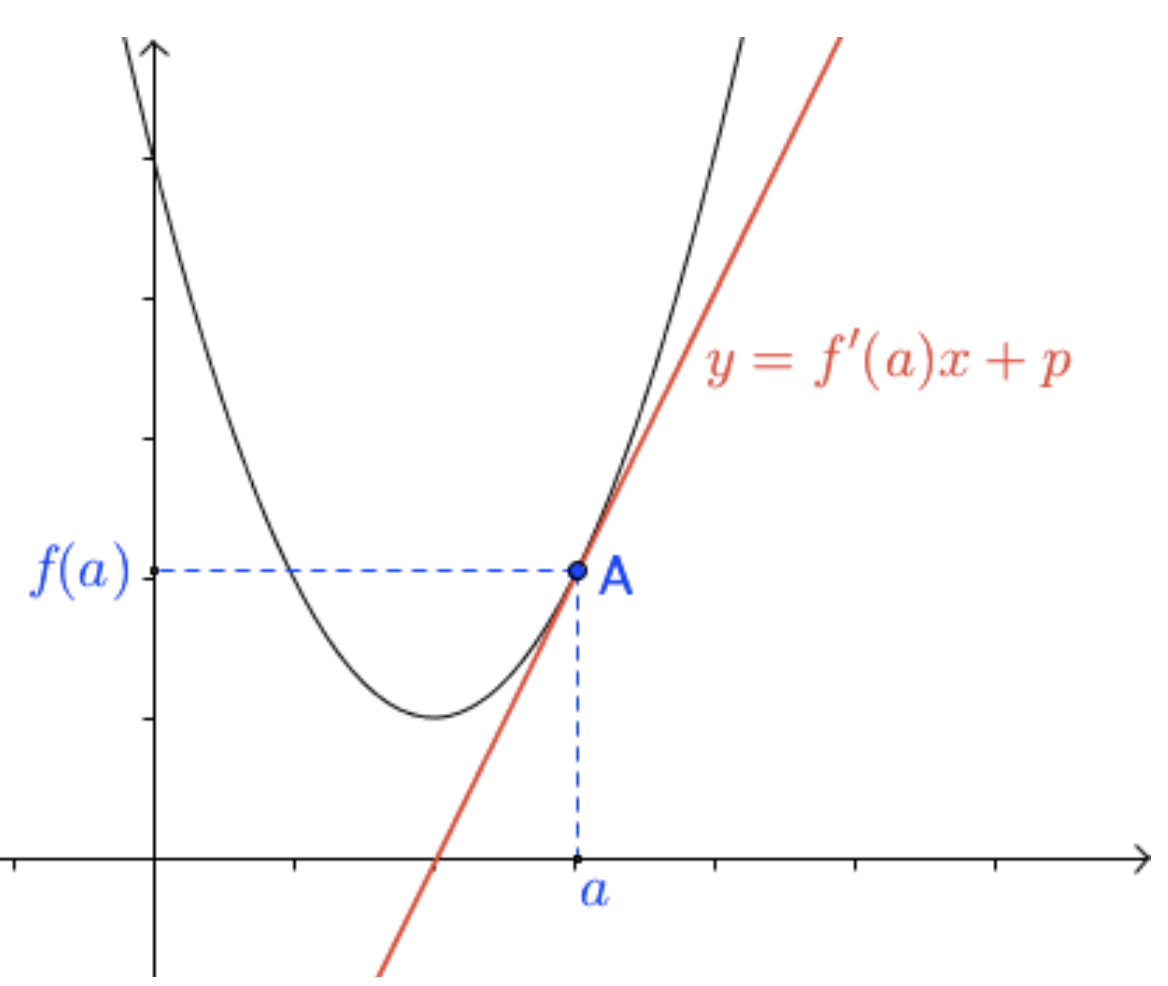
\includegraphics[width=1\textwidth]{coefdirtangente.png}
\end{minipage}%

\newpage
\begin{mdframed}[
    linewidth=1pt,
    roundcorner=5pt,
    linecolor=ForestGreen
]
{\color{ForestGreen}\textbf{Définition :}}
La \textbf{tangente} à la courbe de $f$ au point $A$ d'abscisse $a$ est la droite :
\begin{itemize}
    \item passant par $A$
    \item de \textbf{coefficient directeur} $f'(a)$ (nombre dérivé de $f$ en $a$)
\end{itemize}
\end{mdframed}

\vspace{10pt}

\begin{mdframed}[
    linewidth=1pt,
    roundcorner=5pt,
    linecolor=RoyalBlue,
    innertopmargin=10pt,
    innerbottommargin=10pt
]
{\color{RoyalBlue}\textbf{\underline{Exercice d'application n°3 :} Savoir lire graphiquement 
des nombres dérivés.}}
\vspace{-5pt}
\\
\begin{minipage}[t]{.45\textwidth}%
    \vspace{30pt}
    On a représenté graphiquement la fonction f définie sur $\mathbb{R}$ par $f(x)=-x^2+4x-2$
    ainsi que ses tangentes aux
    points $A$, $B$ et $C$.
    \begin{enumerate}
        \item Déterminer graphiquement $f(0)$, $f(2)$ et $f(3)$
        \item Déterminer graphiquement $f'(0)$, $f'(2)$ et $f'(3)$
        \item Déterminer les équations des droites $T_A$, $T_B$ et $T_C$
    \end{enumerate}
\end{minipage}%
\hfill
\begin{minipage}[t]{.5\textwidth}%
    \vspace{0pt}
    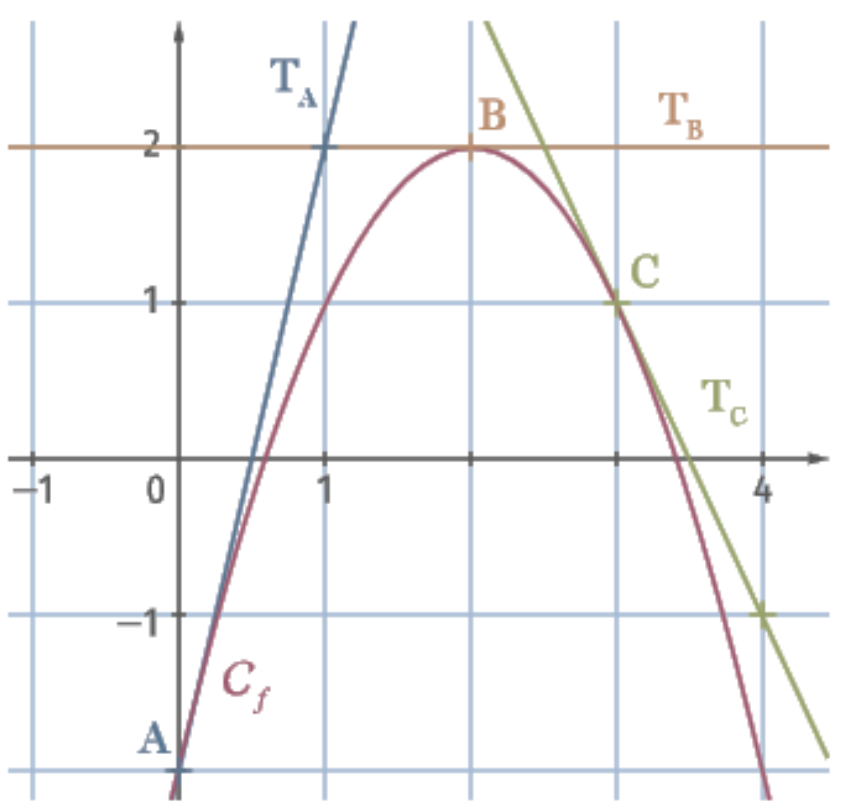
\includegraphics[width=1\textwidth]{exo_tangente_1.png}
\end{minipage}%
\end{mdframed}

\vspace{5pt}

\begin{mdframed}[
    linewidth=1pt,
    roundcorner=5pt,
    linecolor=RoyalBlue,
    innertopmargin=10pt,
    innerbottommargin=10pt
]
{\color{RoyalBlue}\textbf{\underline{Exercice d'application n°4 :} Savoir lire graphiquement 
des nombres dérivés.}}
\vspace{-5pt}
\\
\begin{minipage}[t]{.3\textwidth}%
    \vspace{30pt}
    Sur le graphique ci-contre, $\mathcal{C}_g$ est la courbe représentative de la
    fonction $g$.

    \vspace{10pt}
    $d_1$ est la tangente à $\mathcal{C}_g$ au point $B$ d'abscisse 2
    
    \vspace{5pt}
    $d_2$ est la tangente à $\mathcal{C}_g$ au point $C$ d'abscisse 6

    \vspace{10pt}
    Déterminer graphiquement $f'(2)$ et $f'(6)$.
\end{minipage}%
\hfill
\begin{minipage}[t]{.65\textwidth}%
    \vspace{0pt}
    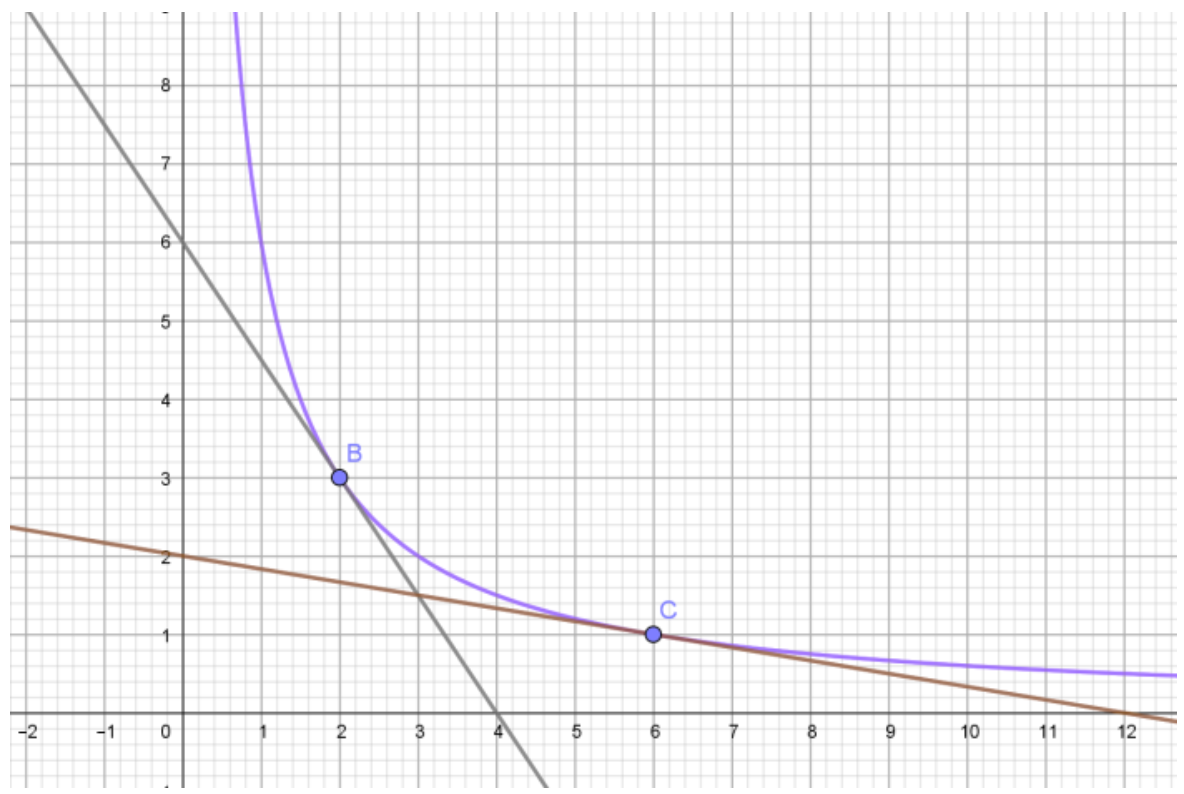
\includegraphics[width=1\textwidth]{exo_tangente_2.png}
\end{minipage}%
\end{mdframed}

\vspace{5pt}

\begin{mdframed}[
    linewidth=1pt,
    roundcorner=5pt,
    linecolor=RoyalBlue,
    innertopmargin=10pt,
    innerbottommargin=10pt
]
{\color{RoyalBlue}\textbf{\underline{Exercice d'application n°5 :} À partir de l'équation 
de la tangente.}}

\vspace{5pt}
La droite d’équation $y=-2x+1$ est la tangente à la
courbe de la fonction $f$ au point \\d’abscisse 2.

\vspace{5pt}
Déterminer $f'(2)$ et $f(2)$.
\end{mdframed}

\vspace{0pt}

% ============================
%   PARTIE 3 : Nombre dérivé
% ============================

\section*{\textcolor{red}{Partie 3 : Dérivée d'une fonction}}

\vspace{10pt}

\begin{mdframed}[
    linewidth=1pt,
    roundcorner=5pt,
    linecolor=ForestGreen
]
{\color{ForestGreen}\underline{\textbf{Définition :}}}

\vspace{5pt}
La fonction qui à tout réel $x$ associe le nombre dérivé de $f$ en $x$ est appelée 
fonction dérivée
de $f$ et se note $f'$.
\end{mdframed}

\begin{mdframed}[
    linewidth=1pt,
    roundcorner=5pt,
    linecolor=red
]
{\color{red}\underline{\textbf{Propriété :}}}

\vspace{5pt}
Les formules de dérivation de fonctions usuelles sont : 
\vspace{-5pt}
\begin{center}
    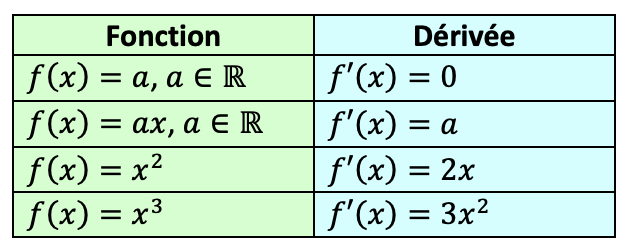
\includegraphics[width=0.5\textwidth]{deriv_usuelles.png}
\end{center}

\textbf{Moyen mnémotechnique : } Pour les puissances de $x$, on vient mettre la puissance
devant le $x$ et on abaisse la puissance de 1.

\vspace{5pt}
    
\end{mdframed}

\begin{mdframed}[
    linewidth=1pt,
    roundcorner=5pt,
    linecolor=red
]
{\color{red}\underline{\textbf{Propriété :}}}

\vspace{5pt}
Les formules d'opérations sur les fonctions dérivées sont : 
\vspace{-5pt}
\begin{center}
    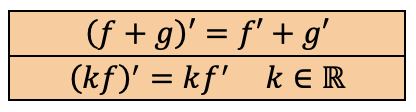
\includegraphics[width=0.33\textwidth]{op_derivees.png}
\end{center}

\end{mdframed}

\begin{mdframed}[
    linewidth=1pt,
    roundcorner=5pt,
    linecolor=RoyalBlue,
    innertopmargin=10pt,
    innerbottommargin=10pt
]
{\color{RoyalBlue}\textbf{\underline{Exercice d'application n°6 :} Calculer des fonctions dérivées.}}
\vspace{5pt}
\\
Dans chaque cas, calculer la fonction dérivée de la fonction $f$ : 
\begin{multicols}{2}
    \begin{enumerate}
        % \setcounter{partno}{2}
        \item $f(x) = 3x$
        \item $f(x) = x^2+5$
    \end{enumerate}
\end{multicols}
\begin{multicols}{2}
    \begin{enumerate}
        \setcounter{enumi}{2}
        \item $f(x) = 5x^3$
        \item $f(x) = 3x^2+4x$
    \end{enumerate}
\end{multicols}
% \begin{enumerate}
%     \item 
% \end{enumerate}
\end{mdframed}

\begin{mdframed}[
    linewidth=1pt,
    roundcorner=5pt,
    linecolor=RoyalBlue,
    innertopmargin=10pt,
    innerbottommargin=10pt
]
{\color{RoyalBlue}\textbf{\underline{Exercice d'application n°7 :}
Calculer la fonction dérivée d'un polynôme de degré 2 ou 3.}}
\vspace{10pt}
\\
Déterminer les fonctions dérivées des fonctions suivantes :
\begin{multicols}{3}
    \begin{enumerate}[label=\alph*)]
        % \setcounter{partno}{2}
        \item $f(x) = 4x^2 - 6x + 1$
        \item $g(x) = x^2 - 2x + 6$
        \item $h(x) = -3x^2 + 2x + 8$
    \end{enumerate}
\end{multicols}
\begin{multicols}{3}
    \begin{enumerate}[label=\alph*)]
        \setcounter{enumi}{3}
        \item $i(x) = x^2 + x + 1$
        \item $j(x) = 5x^2 + 5$
        \item $k(x) = -x^2 + 7x$
    \end{enumerate}
\end{multicols}
\begin{multicols}{2}
    \begin{enumerate}[label=\alph*)]
        \setcounter{enumi}{6}
        \item $l(x) = x^3 - 3x^2 + 2x - 5$
        \item $m(x) = 5x^3 + 2x^2 + 2x - 7$
    \end{enumerate}
\end{multicols}
\begin{multicols}{2}
    \begin{enumerate}[label=\alph*)]
        \setcounter{enumi}{8}
        \item $n(x) = -2x^3-3x^2-7x+8$
        \item $p(x) = -x^3 + x^2 + 1$
    \end{enumerate}
\end{multicols}
\begin{multicols}{2}
    \begin{enumerate}[label=\alph*)]
        \setcounter{enumi}{10}
        \item $r(x) = 4x^3+1$
        \item $s(x) = -x^3 + 7x$
    \end{enumerate}
\end{multicols}
% \begin{enumerate}
%     \item 
% \end{enumerate}
\end{mdframed}


\vspace{20pt}

% ============================
%   PARTIE 4 : Variation d'une fonction polynôme
% ============================

\section*{\textcolor{red}{Partie 4 : Variation d'une fonction polynôme}}

\vspace{10pt}

\begin{mdframed}[
    linewidth=1pt,
    roundcorner=5pt,
    linecolor=red
]
{\color{red}\underline{\textbf{Théorème :}}}

\begin{itemize}
    \item Si $f'(x) \geq 0$ sur un intervalle $I$, alors $\bm{f}$ \textbf{est croissante} sur $I$
    \item Si $f'(x) \leq 0$ sur un intervalle $I$, alors $\bm{f}$ \textbf{est décroissante} sur $I$
    \item Si $f'(x) = 0$ sur un intervalle $I$, alors $\bm{f}$ \textbf{est constante} sur $I$
\end{itemize}

\end{mdframed}

\vspace{5pt}

\underline{Illustration :}

\begin{center}
    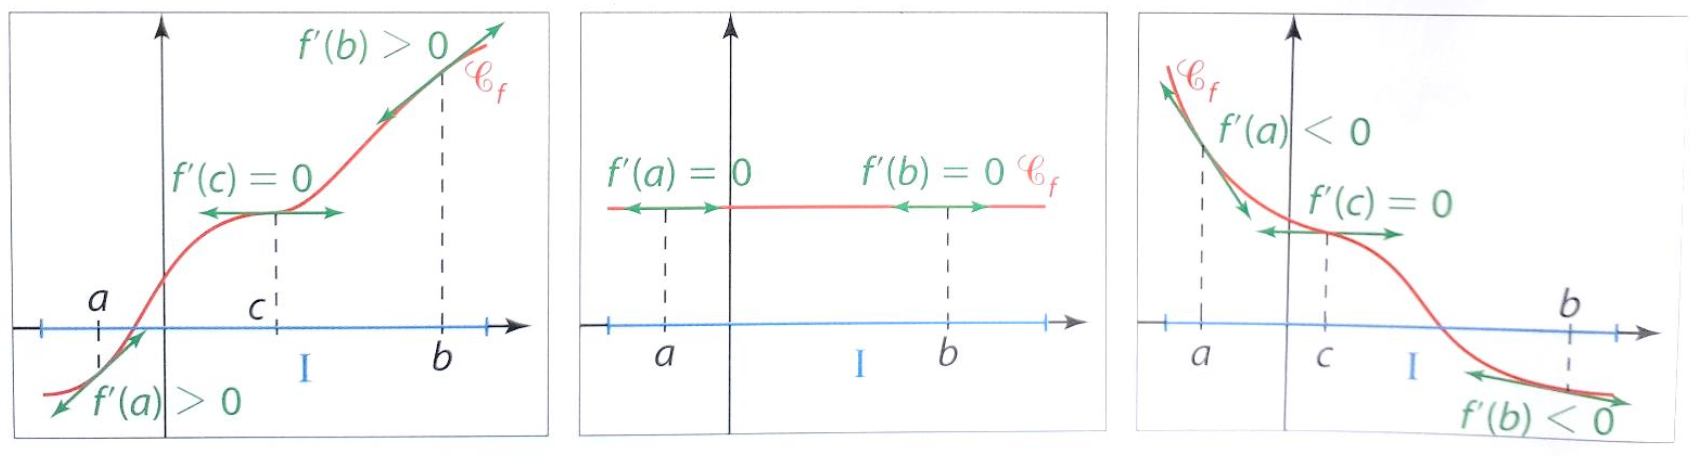
\includegraphics[width=1\textwidth]{variations.png}
\end{center}

\vspace{-15pt}
\textbf{\hspace{1cm}f est croissante sur I \hspace{1.1cm} f est constante sur I 
\hspace{1cm} f est décroissante sur I }

\newpage
\underline{Exemple n°1 :}
\\
\begin{minipage}[t]{.35\textwidth}%
    \vspace{20pt}
    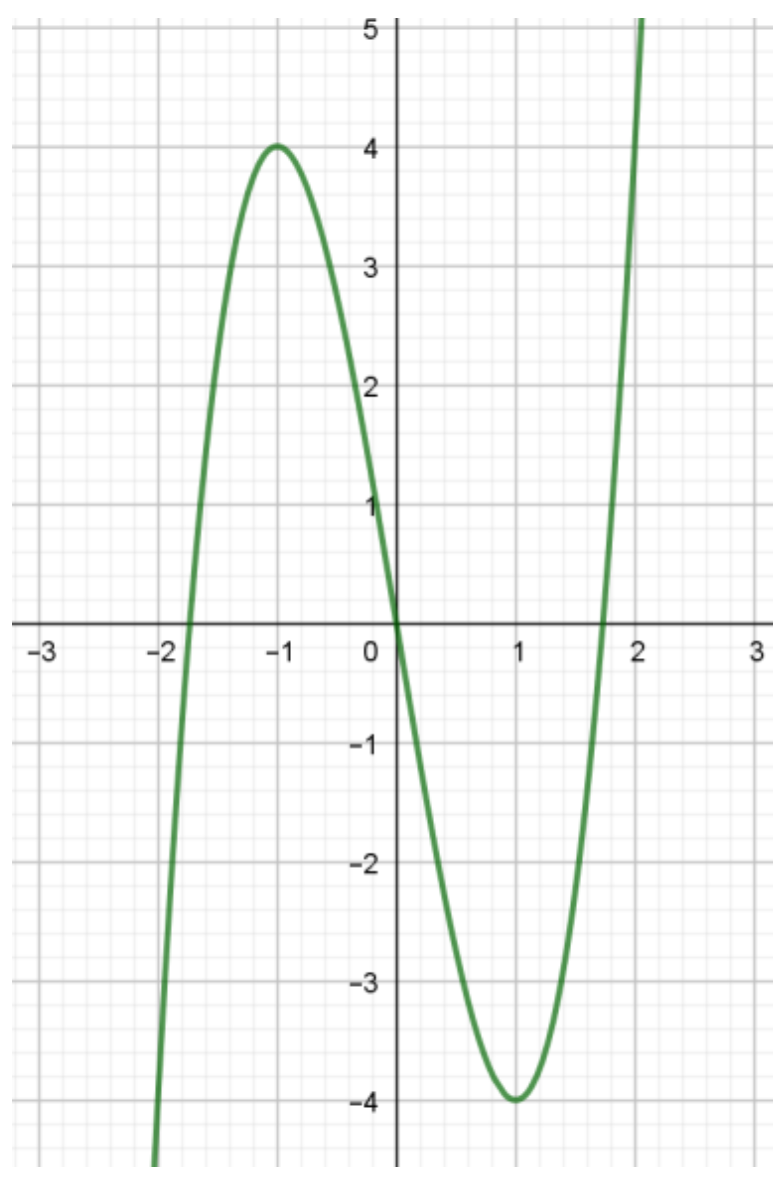
\includegraphics[width=0.9\textwidth]{exemple_variations.png}
\end{minipage}%
\hfill
\begin{minipage}[t]{.65\textwidth}%
    \vspace{0pt}
    La fonction $f$ représentée ci-contre est : 
    
    \vspace{15pt}
    \_\_\_\_\_\_\_\_\_\_\_\_\_\_\_\_ sur \_\_\_\_\_\_\_\_\_\_\_\_\_\_\_

    \vspace{15pt}
    Donc \_\_\_\_\_\_\_\_\_\_\_\_\_\_\_\_\_\_\_\_\_\_\_\_\_\_\_\_\_\_

    \vspace{15pt}
    \_\_\_\_\_\_\_\_\_\_\_\_\_\_\_\_ sur \_\_\_\_\_\_\_\_\_\_\_\_\_\_\_

    \vspace{15pt}
    Donc \_\_\_\_\_\_\_\_\_\_\_\_\_\_\_\_\_\_\_\_\_\_\_\_\_\_\_\_\_\_

    \vspace{10pt}
    On peut résumer ces informations dans le tableau suivant :

    \vspace{10pt}
    $
    \begin{tikzpicture}
    \tkzTabInit[lgt = 3]{$x$ / 1 , Signe de $f'$ / 1, Variations de $f$ / 2}{,,}
    \tkzTabLine{,,,}
    \tkzTabLine{,,,}
    \end{tikzpicture}
    $
\end{minipage}%

\vspace{10pt}

\underline{Exemple n°2 :}

\vspace{10pt}
On considère la fonction $f$ définie sur $\mathbb{R}$ par 
$f(x) = -4x^2 + 3x - 1$

\hspace{1cm}1) On détermine la dérivée de la fonction $f$ :

\vspace{2cm}

\hspace{1cm}2) On étudie le signe de la dérivée :

\vspace{2cm}

\hspace{1cm}2) On en déduit les variations de la fonction $f$ : 

% \vspace{5pt}
\begin{center}
    $
    \begin{tikzpicture}
    \tkzTabInit[lgt = 3]{$x$ / 1 , Signe de $f'$ / 1, Variations de $f$ / 2}{,,}
    \tkzTabLine{,,,}
    \tkzTabLine{,,,}
    \end{tikzpicture}
    $
\end{center}

\begin{mdframed}[
    linewidth=1pt,
    roundcorner=5pt,
    linecolor=RoyalBlue,
    innertopmargin=10pt,
    innerbottommargin=10pt
]
{\color{RoyalBlue}\textbf{\underline{Exercice d'application n°8 :} 
Travailler avec des tableaux.}}
\vspace{5pt}
\\
\begin{minipage}[t]{.4\textwidth}%
    \vspace{0pt}
    Soit $f$ la fonction dérivable sur $\mathbb{R}$ dont le tableau de variation est 
    représenté ci-contre.

    \vspace{10pt}
    Construire le tableau de signes de sa fonction dérivée $f'$.
\end{minipage}%
\hfill
\begin{minipage}[t]{.55\textwidth}%
    \vspace{0pt}
    $
    \begin{tikzpicture}
    \tkzTabInit[espcl = 2]{$x$ / 1 , $f$ / 2}{$-\infty$, $-4$, $5$, $+\infty$}
    \tkzTabVar{-/ , +/ , -/, +/ }
    \end{tikzpicture}
    $
\end{minipage}%

\vspace{30pt}

{\color{RoyalBlue}\textbf{\underline{Exercice d'application n°9 :} 
Travailler avec des tableaux.}}
\vspace{5pt}
\\
Soit $g$ la fonction définie sur $\mathbb{R}$ par $g(x) = x^3 + \dfrac{9}{2}x^2 - 12x + 5$

\vspace{10pt}
\hspace{1cm}1) Calculer la dérivée de $g$
\\

\hspace{1cm}2) Montrer que $g'(x) = 3(x+4)(x-1)$
\\

\hspace{1cm}3) Déterminer le sens de variation de $g$


\end{mdframed}


\end{document}
